\documentclass[xcolor={svgnames},aspectratio=169]{beamer}
\usepackage[english]{babel}
\usepackage{lmodern}
\usepackage{libertinus}
\usepackage{csquotes}
\usepackage{multicol}
\usepackage{caption}
\usepackage{algorithm}
\usepackage{algpseudocode}
\usepackage{comment}
% \usepackage[svgnames]{xcolor} % Must pass direct to beamer class

\usepackage{graphicx}
\makeatletter
\def\input@path{{Chapters/}{other/}{Figures/}{Tables/}}
\makeatother
\graphicspath{{Figures}}
\usepackage[backend=biber,style=ieee,style=authortitle]{biblatex} %authortitle authoryear
\addbibresource{../2025Bibs/Prospectus.bib}
\usepackage{xpatch}
\xapptobibmacro{cite}{\setunit{\nametitledelim}\printfield{year}}{}{}


\title{Working Title}
% \subtitle{A Prospectus Defense}
\author{Capt. Brandon Hosley\inst{1}}
\institute[ENS]{
    \inst{1}
    Department of Operational Sciences\\
    Air Force Institute of Technology}
\date{\today}

\titlegraphic{
    \includegraphics[width=2cm]{afit_logo.png} \hfill
    \includegraphics[width=2cm]{en_logo.png}} 

\AtBeginSection[]{
  \begin{frame}
    \tableofcontents[currentsection, hideothersubsections]
  \end{frame}
}

\usetheme{Montpellier}
\usecolortheme{orchid}
\mode<presentation>

\begin{document}

\frame{\titlepage}
\begin{frame}
    \tableofcontents[subsectionstyle=hide, subsubsectionstyle=hide]
\end{frame}

\section{Introduction}

\begin{frame}{The Vision for Autonomy in Defense}
\begin{columns}
    \begin{column}{0.6\textwidth}
        \begin{itemize}
            \item \textbf{Department of Defense initiatives are actively advancing autonomous 
                system deployment.}
            \begin{itemize}
                \item \textbf{Replicator Initiative:} {Calls for the rapid integration of 
                    commercial-off-the-shelf (COTS) autonomous systems for scalable deployment.
                    \footnotemark[1] } % \footnote[frame]{\cite{robertson2023}} }
                \item \textbf{DARPA's OFFSET:} {Demonstrated feasibility of swarm-enabled ground 
                    and aerial assets in contested environments. 
                    \footnotemark[2] } % \footnote[frame]{\cite{zotero-2835}} }
            \end{itemize}
            \item \textbf{Limitation:} {Reliable autonomy in unpredictable environments 
                remains an unsolved challenge.}
        \end{itemize}
    \end{column}
    \begin{column}{0.4\textwidth}
        \begin{figure}[!h]
            \centering
            \includegraphics[width=0.95\textwidth]{replicator_collage.png}
            \caption{\textbf{Replicator Initiative} aimed at multiple platforms. 
                \footnotemark[1] } % \footnote[frame]{\cite{robertson2023}}}
            \label{fig:replicator_collage}
        \end{figure}
    \end{column}
\end{columns}
\footnotetext[1]{\cite{robertson2023}}
\footnotetext[2]{\cite{zotero-2835}}
\end{frame}


\begin{frame}{Rules-Based Control}
    \begin{itemize}
        \item Traditional autonomous systems operate on hand-coded rules.
        \item Effective in constrained environments with predictable dynamics.
        \item Limitations:
        \begin{itemize}
            \item Brittle under changing conditions.
            \item Poor generalization to novel scenarios.
        \end{itemize}
        \item Led to interest in adaptive learning systems.
    \end{itemize}
\end{frame}

\begin{frame}{Reinforcement Learning (RL)}
    \begin{itemize}
        \item RL enables agents to learn behaviors through trial and error in dynamic environments.
        \item Successes in single-agent settings with clear reward signals and isolated tasks.
        \item Limitations:
        \begin{itemize}
            \item Doesn't scale to multi-agent scenarios without coordination failures.
            \item Learned policies often lack robustness to new agent compositions or input changes.
        \end{itemize}
    \end{itemize}
\end{frame}

\begin{frame}{Multi-Agent RL (MARL)}
    \begin{itemize}
        \item MARL extends RL to scenarios involving multiple learning agents.
        \item Used for both cooperative and competitive environments (e.g., games, simulations).
        \item Limitations:
        \begin{itemize}
            \item Assumes agents are often homogeneous or interchangeable.
            \item High coordination cost and non-stationarity challenges.
        \end{itemize}
    \end{itemize}
\end{frame}

\begin{frame}{Heterogeneous-Agent RL (HARL)}
    \begin{itemize}
        \item HARL addresses coordination among agents with different capabilities, sensors, or roles.
        \item Promising for real-world applications with diverse platforms (e.g., COTS drones, mixed teams).
        \item Limitations:
        \begin{itemize}
            \item Limited scalability in training architectures.
            \item Fragile under observation or team composition changes.
        \end{itemize}
    \end{itemize}
\end{frame}

\begin{frame}{Open Challenges in Scalable Multi-Agent Autonomy}
    \begin{itemize}
        \item Integration across heterogeneous platforms is constrained by inflexible model assumptions.
        \item Retraining cost grows rapidly with team size and complexity.
        \item Teams struggle to adapt dynamically to changing sensors or agent availability.
        \item Existing strategies for curriculum learning and network scaling are underdeveloped.
    \end{itemize}
\end{frame}



\begin{frame}{Why Heterogeneous Autonomy Matters}
\begin{columns}
    \begin{column}{0.6\textwidth}
    \begin{itemize}
        \item \textbf{Operational autonomy must account for platform diversity.}
        \begin{itemize}
            \item Teams may integrate UAVs and UGVs with different sensors, dynamics, and connectivity constraints.
            \item Heterogeneous-agent reinforcement learning (HARL) enables coordination across dissimilar platforms.
        \end{itemize}
        \item \textbf{Policy transfer and input-invariant networks} can support:
        \begin{itemize}
            \item Adaptability to new team compositions.
            \item Resilience to partial observation loss or sensor degradation.
        \end{itemize}
    \end{itemize}
    \end{column}
    \begin{column}{0.4\textwidth}
        \begin{figure}[!h]
            \centering
            \includegraphics[width=0.95\textwidth]{offset_collage.jpg}
            \caption{\textbf{OFFSET} test platforms.
                \footnote[frame]{\cite{zotero-2835}}}
            \label{fig:offset_collage}
        \end{figure}
    \end{column}
\end{columns}
\end{frame}


% Research Contributions
\begin{frame}{Research Contributions}
    \begin{itemize}
        \item {% Through-line:
            Advance the study of heterogeneous-agent reinforcement learning by exploring 
            scalable training architectures and policy designs that support adaptability 
            to agent diversity and team variation.}
        \item {% Contribution 1:
            Evaluate a policy upsampling strategy for training larger multi-agent teams 
            more efficiently using pretrained smaller-team policies.}
        \item {% {Contribution 2:
            Investigate input-invariant policy architectures for shared learning and 
            robustness in teams of heterogeneous agents.}
        \item {% Contribution 3: 
            Design and evaluate a curriculum that progressively expands network capacity 
            via tensor projection to improve training efficiency.}
    \end{itemize}
\end{frame}

\begin{frame}{Research Objectives}
    \textbf{Contribution 1}
    % \textbf{Contribution 1 - Direct Scaling of Teams}
    \begin{itemize}
        \item {Improve training efficiency by scaling teams from smaller pretrained groups 
            using policy duplication instead of retraining from scratch.}
        \item {Demonstrate that policy reuse across increasing agent counts can reduce 
            training cost while maintaining performance.}
    \end{itemize}
    \vspace{1em}
    \textbf{Contribution 2}
    % \textbf{Contribution 2 - Input-Invariant Policy Architectures}
    \begin{itemize}
        \item {Construct input-invariant policy architectures to enable shared training 
            updates across agents with heterogeneous observation structures.}
        \item {Evaluate the effectiveness of input-invariant models in improving learning 
            efficiency in teams with overlapping observations.}
        \item {Test whether these models maintain stable performance under dynamic 
            observation space changes during execution.}
    \end{itemize}
\end{frame}

\begin{frame}{Research Objectives}
    \textbf{Contribution 3}
    % \textbf{Contribution 3 - Progressive Network Growth via Tensor Projections}
    \begin{itemize}
        \item {Demonstrate the feasibility of expanding a policy network mid-training 
            using tensor projection without discarding prior knowledge.}
        \item {Identify when during training such growth provides learning advantages 
            over fixed-size architectures.}
        \item {Compare performance and efficiency of progressive-growth networks to 
            fixed-size baselines in terms of convergence and cost.}
    \end{itemize}
\end{frame}


\section{Contribution 1}

% For each Contribution:
% Re-motiviate
%     Introduction
%         Lit review
%         Contribution
%     Methodology
%     Experimental Procedure
%     Results
%     Discussion

\subsection{Introduction}

\begin{frame}
\end{frame}

\subsubsection{Literature Review}

\subsubsection{Research Questions}

\begin{frame}{Research Questions}
    \begin{enumerate}
        \item[RQ 1] {
            Can pretraining smaller teams of agents and then scaling to the target 
            team size via policy duplication and retraining improve training efficiency 
            without sacrificing final policy performance in MARL?}
        \item[RQ 2] {
            How does the effectiveness of this direct scaling strategy vary across 
            environments with different forms of agent heterogeneity 
            (e.g., behavioral vs. intrinsic)?}
    \end{enumerate}
\end{frame}

\begin{frame}{RQ 1 - Research Tasks}
    \begin{enumerate}
        \item[RQ 1] \textcolor{gray}{
            Can pretraining smaller teams of agents and then scaling to the target 
            team size via policy duplication and retraining improve training efficiency 
            without sacrificing final policy performance in HARL? } \vspace{1em}
    \begin{itemize}
        \item[RT 1.1] {
            Design an upsampling-based curriculum using policy duplication and retraining.}
        \item[RT 1.2] {
            Define a metric (agent-steps) accounting for agent count and training time.}
        \item[RT 1.3] {
            Train tabula rasa agents each target environment and team size as baselines.}
        \item[RT 1.4] {
            Evaluate training performance across various pretraining length and target team sizes.}
    \end{itemize}
    \end{enumerate}
\end{frame}

\begin{frame}{RQ 2 - Research Tasks}
    \begin{enumerate}
        \item[RQ 2] \textcolor{gray}{
            How does the effectiveness of this direct scaling strategy vary across 
            environments with different forms of agent heterogeneity 
            (e.g., behavioral vs. intrinsic)? } \vspace{1em}
    \begin{itemize}
        \item[RT 2.1] {
            Select environments that represent distinct forms of agent heterogeneity. \\
            Behavioral, Intrinsic.}
        \item[RT 2.2] {
            Adapt observation structures to enable fixed policy architectures across team sizes.}
        \item[RT 2.3] {
            Evaluate the effect of heterogeneity type on the scalability and retraining benefit.}
    \end{itemize}
    \end{enumerate}
\end{frame}

% \subsection{Methodology}
% \subsection{Experimental Procedure}
% \subsection{Results}
% \subsection{Discussion}
\section{Contribution 2}

% For each Contribution:
%     Introduction
%         Recall Motivation
%         Lit review
%         Contribution
%     Methodology
%     Experimental Procedure
%     Results
%     Discussion

\subsection{Introduction}

\begin{frame}{The Case for Input-Invariant Architectures}
    \begin{itemize}
        \item Heterogeneous agent teams frequently encounter differences in observation 
            structure due to varying sensor suites and mission roles.
        \item Traditional policy networks require fixed, consistent inputs—limiting their 
            ability to scale or adapt.
        \item Input-invariant architectures offer a promising alternative by allowing 
            policies to generalize across agents and configurations without retraining.
        \item This contribution explores how these architectures can improve learning 
            efficiency and robustness in dynamic, real-world team settings.
    \end{itemize}
\end{frame}


\subsubsection{Literature Review}


\begin{frame}{Theoretical Foundations}
    \textbf{Exchangeability and Symmetry}
    \begin{itemize}
        \item \textbf{de Finetti's Theorem:} Exchangeable sequences behave like i.i.d. 
            draws from a latent distribution~\footcite{alvarez-melis2015}.
        \item In MARL, agent observations are often unordered—motivating 
            \textbf{permutation-invariant} architectures.
        \item \textbf{Key Insight:} Architectures that respect symmetry in input 
            ordering can improve generalization and efficiency~\footcite{hartford2018}
            for exchangeable agents.
    \end{itemize}
\end{frame}

\begin{frame}{Permutation Invariance and Equivariance}
    \textbf{Deep Sets} \footcite{zaheer2017}
    \begin{itemize}
        \item Any permutation-invariant function can be expressed in terms of 
            a transformation \(\phi\) over elements and a transformation \(\rho\) of the sum: 
            \[\rho\left(\sum_i \phi(x_i)\right)\]
        \item Zaheer et al. use shared parameters through constrained weight matrices.
        \begin{itemize}
            \item With all off-diagonal elements \(\gamma\)
            \item Diagonal elements \(\lambda+\gamma\)
        \end{itemize}
        \item \textbf{Implication:} Enables parameter sharing across agents with unordered observations.
        \item Improves sample efficiency and scalability in symmetric MARL settings.
    \end{itemize}
\end{frame}

\begin{frame}{Mean-Field Methods and Exchangeability}
    \textbf{From Aggregation to Generalization}
    \begin{itemize}
        \item Replace summation with \textbf{averaging} to make outputs insensitive to agent count.
        \item \textbf{Mean-Field MARL}~\footcite{yang2018}: 
            Use average of neighbors in actor and critic networks.
        \item MF-PPO achieves~\footcite{li2021b}:
        \begin{itemize}
            \item Convergence rates independent of team size
            \item Superior performance and reduced model complexity
        \end{itemize}
        \item \textbf{Limitation:} Subset-specific interaction information may be lost.
    \end{itemize}
\end{frame}

% \begin{frame}{Graph-Based Architectures}
%     \textbf{Relational Inductive Bias}
%     \begin{itemize}
%         \item Graph Neural Networks (GNNs) treat agents as nodes; edges represent interactions.
%         \item \textbf{IHG-MA} \footcite{yang2021a}: Dynamic agent graphs with shared policies.
%         \item \textbf{PIC} \footcite{liu2020b}: Graph critic pooled over agents, scalable to 200 agents.
%         \item Attribute embeddings encode agent roles or types, enabling heterogeneous agent support.
%     \end{itemize}
% \end{frame}

\begin{frame}{Attention for Set-Based Inputs}
    \begin{columns}
        \begin{column}{0.6\textwidth}
            \textbf{Transformers and Self-Attention}
            \begin{itemize}
                \item Attention layers (without positional encodings) are naturally permutation-invariant.
                \item \textbf{Set Transformer} \footcite{lee2019}: 
                    Captures high-order relationships among unordered elements.
                \item \textbf{MAAC} \footcite{iqbal2019}: 
                    Attention-weighted centralized critic for better credit assignment.
                \item Applied to large-scale MARL tasks (e.g., SMAC) with strong results.
            \end{itemize}
        \end{column}
        \begin{column}{0.4\textwidth}
            \begin{figure}
                \includegraphics[width=0.85\linewidth]{C2/lee2019_set_transformer.png}
                \caption{Set Transformer model by Lee et al~\footcite{lee2019}.}
            \end{figure}
        \end{column}
    \end{columns}
\end{frame}

\begin{frame}{Single-Agent Generalization}
    \begin{columns}
        \begin{column}{0.6\textwidth}
            \textbf{Lessons Beyond MARL}
            \begin{itemize}
                \item \textbf{Zambaldi et al.} \footcite{zambaldi2018}: 
                    Graph-based reasoning improves single-agent performance in StarCraft II.
                \item \textbf{Tang and Ha} \footcite{tang2021}: 
                    Sensory-channel invariance enables robustness to occlusion and dropout.
                \item Treating input channels as exchangeable improves perceptual robustness.
            \end{itemize}
        \end{column}
        \begin{column}{0.4\textwidth}
            \begin{figure}
                \includegraphics[width=0.95\linewidth]{C2/tang2021_view.png}
                \caption{Original and permuted image inputs used by Tang and Ha~\footcite{tang2021}.}
            \end{figure}
        \end{column}
    \end{columns}
\end{frame}

\begin{frame}{Toward Heterogeneous MARL}
    \begin{columns}
        \begin{column}{0.6\textwidth}
            \textbf{Challenges in Heterogeneous-Agent Learning}
            \begin{itemize}
                \item Input-invariant methods often assume identical agent observation distributions.
                \item \textbf{Strategy:} Augment observations with role/type embeddings.
                \item \textbf{HPN} \footcite{hao2023}: Hypernetworks generate role-conditioned modules.
                \item \textbf{Open Question:} What are the tradeoffs in cost and complexity vs. performance?
            \end{itemize}
        \end{column}
        \begin{column}{0.4\textwidth}
            \begin{figure}
                \includegraphics[width=\linewidth]{C2/hao2022_network_overview.png}
                \caption{Hao et al's PI and PE policy network overview~\footcite{hao2023}.}
            \end{figure}
        \end{column}
    \end{columns}
\end{frame}

\begin{frame}{Summary of Key Ideas}
\begin{itemize}
    \item Input-invariance enables better generalization and efficiency in symmetric multi-agent settings.
    \item Mean-field, GNNs, and attention each offer scalable strategies with tradeoffs in specificity and complexity.
    % \item Extensions to HARL require mechanisms to encode agent roles/types while preserving symmetry when possible.
    \item Empirical comparisons of cost vs. benefit are still lacking in literature.%—this work aims to address that.
\end{itemize}
\end{frame}

\subsubsection{Research Questions}

\begin{frame}{Contribution 2 - Research Questions}
    \begin{enumerate}
        \item[RQ 1] {
            How does incorporating input-invariant structures \emph{(i.e., networks 
            that are robust to feature permutation and input length differences)}
            into policy networks affect learning efficiency and team robustness 
            when heterogeneous agents have partially overlapping observation spaces?
            }
        \item[RQ 2] {
            Do input-invariant architectures lead to more stable policy performance under 
            team-size changes and partial observation loss during execution?
            }
        \item[RQ 3] {
            What are the computational and implementation costs of mean-field
            architectures relative to their performance benefits?
            }
    \end{enumerate}
\end{frame}

\begin{frame}{RQ 1 - Research Tasks}
    \begin{enumerate}
        \item[RQ 1] \textcolor{gray}{
            How does incorporating input-invariant structures \emph{(i.e., networks 
            that are robust to feature permutation and input length differences)}
            into policy networks effect learning efficiency and team robustness 
            when heterogeneous agents have partially overlapping observations? } \vspace{1em}
    \begin{itemize}
        \item[RT 1.1] {
            Design and implement a policy architecture that exhibits input-invariance through 
            techniques such as pooling layers, attention mechanisms, or permutation-invariant 
            encodings.}
        \item[RT 1.2] {
            Identify benchmark environments where agents possess distinct but partially 
            overlapping observation features (e.g., different sensor arrays).}
        \item[RT 1.3] {
            Train these, input-invariant policy networks in the selected setting(s) and measure 
            learning rate and convergence behavior.}
        \item[RT 1.4] {
            Compare input-invariant shared architectures against baseline (non-invariant) 
            architecture to evaluate performance and learning benefits.}
    \end{itemize}
    \end{enumerate}
\end{frame}

\begin{frame}{RQ 2 - Research Tasks}
    \begin{enumerate}
        \item[RQ 2] \textcolor{gray}{
            Do input-invariant architectures lead to more stable policy performance under 
            team-size changes and partial observation loss during execution? } \vspace{1em}
    \begin{itemize}
        \item[RT 2.1] {
            Simulate runtime degradation by selectively masking subsets of agent observations 
            (e.g., sensor failure) for both the input-invariant and baseline policy models.}
        \item[RT 2.2] {
            Simulate dynamic changes in team size by removing agents during evaluation 
            in both the input-invariant and baseline policy models.}
        \item[RT 2.3] {
            Measure policy stability, reward degradation, and recovery behavior under these 
            perturbations for both the input-invariant and baseline models.}
        \item[RT 2.4] {
            Statistically compare performance between input-invariant and baseline models 
            across all perturbation conditions to assess resilience and stability.}
    \end{itemize}
    \end{enumerate}
\end{frame}

\begin{frame}{RQ 3 - Research Tasks}
    \begin{enumerate}
        \item[RQ 3] \textcolor{gray}{ 
            What are the computational and implementation costs of mean-field
            architectures relative to their performance benefits? }
        \vspace{1em}
        \begin{itemize}
            \item[RT 3.1] {
                Benchmark computational cost during training and 
                inference (e.g., agent-steps, step-costs).}
            \item[RT 3.2] {
                Perform Statistical comparison of relative training cost, rate of convergence, 
                in training and rate of performance degradation in completed models.}
        \end{itemize}
    \end{enumerate}
\end{frame}

\subsection{Methodology}

\subsubsection{Environment Model}

\begin{frame}{Environment Model (RT 1.2)}
    Using Powell's~\footcite{powell2022}
    framework for modeling:
    \begin{columns}
        \begin{column}{0.3\linewidth}
            \begin{enumerate}
                \item State
                \item Decision/Action
                \item Exogeneous Information
                \item Transition Function
                \item Objective Function
            \end{enumerate}
        \end{column}
        \begin{column}{0.7\linewidth}
        \end{column}
    \end{columns}
\end{frame}


\begin{frame}{State: Time and Joint Representation}
    \begin{itemize}
        \item Let \(T\subset\mathbb{N}\) be the set of decision epochs.
        \item Let entities \(E := (I, J, K, L)\), where:
        \begin{itemize}
            \item \(i\in I\): agents
            \item \(j\in J\): objectives
            \item \(k\in K\): hazards
            \item \(l\in L\): obstacles
        \end{itemize}
        \item For time period \(t\in T\) and entities \(e\in E\), the joint state is:
        \[
            s_t := \{s_{te}\ \forall\ e\in E\}, \quad s_t \in S
        \]
    \end{itemize}
\end{frame}

\begin{frame}{State: Marginal Representations}
    Let \(N\in \mathbb{N}\) be the number of spatial dimensions,
    and for each \(n \in \{1, \dots, N\}\),
    let \(D^{(n)} \in \mathbb{F}\) denote the domain of the \(n\)th dimension.
    % Let,
    % \begin{itemize}
    %     \item \(N\in \mathbb{N}\) be the number of spatial dimensions.
    %     \item  and for each \(n \in \{1, \dots, N\}\), 
    %         let \(D^{(n)} \in \mathbb{F}\) denote the domain of the \(n\)th dimension.
    % \end{itemize}
    Then for,
    \begin{itemize}
        \item non-agents \(e\in (J, K, L)\) marginal states are: \vspace{-0.8em}
        \[
            s_{te} := (d_{te})
        \]
        \item agents \(i\in I\) marginal states are: \vspace{-0.8em}
        \[
            s_{ti} := (d_{ti}, \theta_{ti})
        \]
    \end{itemize}
    Where.
    \begin{itemize}
        \item the location vector is: \vspace{-0.8em}
        \[
            d_{te} := \left(d_{te}^{(1)},\ldots, d_{te}^{(N)}\right) \in \prod_{n=1}^{N} D_{e}^{(n)}
        \]
        \item and the orientation vector is: \vspace{-0.8em}
        \[
            \theta_{ti} := \left(\theta_{ti}^{(1,2)},\ldots, \theta_{ti}^{(N-1,N)}\right) \in \prod_{n=1}^{N-1} \Theta_{i}^{(n,n+1)}
        \]
    \end{itemize}
\end{frame}

\begin{frame}{Decision/Action}
    Joint action \(a \in A\) is the combination of agent's actions \(a_i\).
    \[
        a := \left(a_{1}, \ldots, a_{|I|}\right) \ \in A := \prod_{i\in I}^{} A_i
    \]
    Then the marginal action space for agent \(i\in I\) is,
    \[
        a_{ti}^{} := (a_{ti}^\text{interact},a_{ti}^\text{move},\Delta\theta_{ti})
    \]
    where,
    \begin{itemize}
        \item \(a_{ti}^\text{interact} \in \{0,1\}\) indicates whether the agent will attempt 
            to interact with the environment (1 = interact, 0 = no interaction),
        \item \(a_{ti}^\text{move} \in M_i \subseteq \mathbb{F}\) 
            denotes the forward movement magnitude of agent \(i\),
        \item \(\Delta\theta_{ti} := \left(\Delta\theta_{ti}^{(1,2)},\ldots, 
            \theta_{ti}^{(N-1,N)}\right) \in \prod_{n=1}^{N-1} \Delta\Theta_{i}^{(n,n+1)}\) 
            specifies the adjustments to the agent's orientation along each rotational axis.
    \end{itemize}
\end{frame}

\begin{frame}{Heterogeneous Action Spaces}
    Heterogeneous action spaces can be naturally modeled through constraints on action spaces:
    \begin{columns}[T]
        \begin{column}{0.5\textwidth}
            \begin{itemize}
                \item \textbf{Movement:} for \(a_{ti}^\text{move} \in M_i \subseteq \mathbb{F}\)
                \item \textbf{Orientation Adjustment:} in general,
                    \[
                        \Delta\Theta_i := \left\{ k \cdot \delta_{\theta_i} 
                        \mid k \in \mathbb{F},\ |\delta_{\theta_i} k| \leq \pi \right\}
                    \]
                where \(k \in [-1,1] \subset \mathbb{F}\) is the range of allowable adjustment
                and \(\delta\) is the resolution of the adjustment 
            \end{itemize}
        \end{column}
        \begin{column}{0.5\textwidth}
            \textbf{A Gridworld Example:}
                \begin{itemize}
                    \item \(\delta := \frac{\pi}{2}\) for ortholinear constraint
                    \item \(\delta := \frac{\pi}{4}\) allows diagonal movement
                    \item A \textbf{rotary-wing aircraft} 
                    \begin{itemize}
                        \item \(M_i := \{0,1\}\)
                        \item \(k_i \in \mathbb{Z} \equiv \{-4, \ldots, 4\} \)
                    \end{itemize}
                    \item A \textbf{fixed-wing aircraft}
                    \begin{itemize}
                        \item \(M_i := \{1,2\}\)
                        \item \(k_i \in \{-1,0,1\}\)
                    \end{itemize}
                \end{itemize}
        \end{column}
    \end{columns}
\end{frame}

\begin{frame}{Exogeneous Information}
    Currently this representation is
    \begin{itemize}
        \item Complete Information: known reward
        \item Imperfect Information: partially observable environment
    \end{itemize} 
    \textbf{Future-work fodder}: An implementation in which channels convey probabilistic 
    information would change this to a incomplete information (and Bayesian) game.
\end{frame}

\begin{frame}{Transition Function}
    This model is deterministic and progresses with agent decisions executed in parallel.\\[1em]
    Thus, the environment transition from state \(s_t\) under joint action \(a_t\) is:
    \[
        s_{t+1} = \mathcal{T}(s_t, a_t)
    \]
    or equivalently, in conditional form:
    \[
        \mathcal{T}(a_t \mid s_t) = s_{t+1}
    \]
\end{frame}

\begin{frame}{Objective Function}
    The objective is to optimize behavior by:
    \begin{itemize}
        \item Max \(\mathcal{R}(j) = r_{j} \in \mathbb{R}_{>0}\) the reward for collecting objective \(j\),
        \item Min \(\mathcal{R}(i) = r_{i} \in \mathbb{R}_{<0}\) the penalty for interaction use by agent \(i\),
        \item Min \(\mathcal{R}(k) = r_{k} \in \mathbb{R}_{<0}\) the penalty for proximity to hazard \(k\).
    \end{itemize}
    Then, the cumulative objective is:
    % {\footnotesize
    % \begin{align*}
    %     \max \sum_{t\in T} &\left[
    %         \sum_{i\in I, j\in J} r_{j} \cdot \mathbb{I}\left[
    %             \|d_{ti}-d_{tj}\| \leq i^\text{range} 
    %             \land \left| \tan\theta_{ti}^{(n,n+1)} - \frac{d_{tj}^{(n+1)}-d_{ti}^{(n+1)}}{
    %                 d_{tj}^{(n)}-d_{ti}^{(n)}} \right| \leq \epsilon 
    %             \land a_{ti}^\text{interact} = 1 
    %         \right] 
    %     \right. \\
    %     &\left.
    %         \quad - \sum_{i\in I} r_{i} \cdot \mathbb{I}\left[a_{ti}^\text{interact} = 1\right]
    %         - \sum_{i\in I, k\in K} r_{k} \cdot \mathbb{I}\left[\|s_{ti} - s_{tk}\|_\infty 
    %         \leq k^\text{range}\right]
    %     \right]
    % \end{align*}}
    \[ 
        \max \sum_{t\in T} \left[
            \sum_{i\in I, j\in J} r_{j} \cdot \mathbb{I}\left[ \Xi \right]
            - \sum_{i\in I} r_{i} \cdot \mathbb{I}\left[a_{ti}^\text{interact} = 1\right]
            - \sum_{i\in I, k\in K} r_{k} \cdot \mathbb{I}\left[\|s_{ti} - s_{tk}\|_\infty
            \leq k^\text{range}\right]
        \right]
    \]
    Where $\Xi$ represents the conditions of objectives.
\end{frame}

\begin{frame}{Objective Conditions}
    \(\mathbb{I}[\Xi]\) is a function representing the conditions of objectives.
    A basic example:
    \begin{align*}
        \Xi := &\,\ a_{ti}^\text{interact} = 1 && \text{Did agent \(i\) try to interact?} \\ 
        & \land \|d_{ti}-d_{tj}\| \leq i^\text{range} &&\text{Is \(j\) in range of agent \(i\)?}\\
        & \land \left| \tan\theta_{ti}^{(n,n+1)} 
            - \frac{d_{tj}^{(n+1)}-d_{ti}^{(n+1)}}{d_{tj}^{(n)}-d_{ti}^{(n)}} \right| 
            \leq \epsilon && \text{Is \(i\) facing \(j\)?}
    \end{align*}
    Additional conditions likely to consider:
    \begin{itemize}
        \item Min number of agents needed to cooperate
        \item Sum of agent levels exceeds an objective difficulty
        \item Some abstract type matching
    \end{itemize}
\end{frame}

\subsubsection{Observation Model}

\begin{frame}{Observation Model}
    In this subsection:
    \begin{itemize}
        \item Imperfect Information Game
        \item Channels Representing States
        \item Modeling Heterogeneous Observation Space
        \item Intuition for a Heterogeneous Observation Space
    \end{itemize}
\end{frame}

\begin{frame}{Imperfect Information}
    \begin{columns}
        \begin{column}{0.4\linewidth}
            This an imperfect information game resulting from partial observability.
            \\[1em]
            Thus, for agent \(i\), an observation \(o_i\) is a function of the state:
            \[o_{ti} = \mathcal{O}_{i}(s_{t}) .\]
        \end{column}
        \begin{column}{0.5\linewidth}
            \begin{figure}
                \begin{subfigure}[t]{0.45\textwidth}
                    \includegraphics[width=\textwidth]{screen_minigrid}
                    \caption{View-range of agent in Minigrid~\footcite{chevalier-boisvert2023}.}
                \end{subfigure}
                \hfill
                \begin{subfigure}[t]{0.45\textwidth}
                    \includegraphics[width=\textwidth]{screen_lbf}
                    \caption{View-range of agent pair in Level-based Foraging~\footcite{papoudakis2021}.}
                \end{subfigure}
            \end{figure}
        \end{column}
    \end{columns}
\end{frame}

\begin{frame}{Channels for Binary Mapping}
    \begin{columns}
        \begin{column}{0.6\linewidth}
            Specific entities are represented by channels:
                \begin{itemize}
                    \item An observation is a set of one-hot matrices
                    \item One matrix per type of entity
                \end{itemize}
            Pursuit example channels:
                \begin{itemize}
                    \item For \(e\in E := \{\text{Friend, Foe, Barrier}\}\)
                    \item Then state \(s\)
                \end{itemize}
                \[s = \{0,1\}^{E\times D_1\times D_2}\]
        \end{column}
        \begin{column}{0.4\linewidth}
            \begin{figure}
                \includegraphics[width=0.65\linewidth]{screen_pursuit_channels.png}
                \caption{Observation Channels in Pursuit~\footcite{gupta2017}.}
            \end{figure}
            \centering
        \end{column}
    \end{columns}
\end{frame}

\begin{frame}{Heterogeneous Observation Channels}
    For heterogeneous observation channels \(C\),
    visibility of entities \(E\) is, may be considered a
    trait of \(e\):
    \[
        e^{(c)} \in \{\text{True, False}\}.
    \]
    But more flexibly, this may be modeled 
    as a sort of categorical dimension of the state:
    \[
        s_{tec} = 
        \begin{cases}
            1& \text{if \(e\) is visible in \(c\)} \\ 
            0& \text{if \(e\) is not visible in \(c\)}
        \end{cases} 
        \quad\forall t\in T, e\in E, c\in C.
    \]
    regardless of if \(e\)'s visibility in \(c\) is expected to change.
\end{frame}

\begin{frame}{Heterogeneous Observation Channels}
    The addition of the observation channels modifies
    entity state in general to:
    \[s_{te} :(c_{te},d_{te}).\]
    and agent state in particular to:
    \[s_{ti} :(c_{ti},d_{ti},\theta_{ti}).\]

    Similar to Pursuit, our model can be represented as a binary mapping
    and extended with Heterogeneous channels \(c\in C\) as:
    \[
        S = \{0,1\}\exp\left(|C|\times E_\text{types}
        \times \prod_{n}^{N} D_n \times \prod_{n}^{N-1} \theta_n\right),
    \]
\end{frame}

\begin{frame}{Intuition for Heterogeneous Observation}
    Let \(C = \{\text{Red, Blue, Green}\}\).
    Then, the RGB color model 
    provides a convenient shorthand for multiple truths. \\
   \begin{figure}
        \centering
        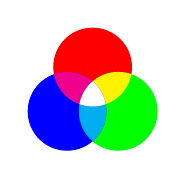
\begin{tikzpicture}
    \def\di{0.5}
    \def\si{0.75*\di}
    \draw [draw=none, fill=red] (90:\si) circle (\di);
    \draw [draw=none, fill=green] (-30:\si) circle (\di);
    \draw [draw=none, fill=blue] (210:\si) circle (\di);
    \begin{scope} % red + green = yellow
        \clip (90:\si) circle(\di);
        \draw [draw=none, fill=yellow] (-30:\si) circle (\di);
    \end{scope} % blue + red = magenta
    \begin{scope}
        \clip (210:\si) circle(\di);
        \draw [draw=none, fill=magenta] (90:\si) circle (\di);
    \end{scope}
    \begin{scope} % green + blue = cyan
        \clip (-30:\si) circle(\di);
        \draw [draw=none, fill=cyan] (210:\si) circle (\di);
    \end{scope}
    \begin{scope} % red + green + blue = white
        \clip (90:\si) circle(\di);
        \clip (210:\si) circle(\di);
        \draw [draw=none, fill=white] (-30:\si) circle (\di);	
    \end{scope}
\end{tikzpicture}
    \end{figure}
    Then, in the next slide we present a Minigrid-like state made heterogeneous.
\end{frame}

\begin{frame}{An Example State}
    \begin{columns}
        \begin{column}{0.4\linewidth}
            Legend:
            \begin{figure}
                \resizebox{!}{0.5\linewidth}{%
                    \NewDocumentCommand{\drawgrid}{O{black} O{8} O{#2}}{%
    % #1 = color (optional, defaults to black)
    % #2 = size (e.g., 8 for 8x8)
    % #3 = second size (e.g., 4 for 8x4)
    \foreach \i in {0,...,#2} {%
        \draw[thin, color={#1}] (\i,0) -- (\i,#3);}
    \foreach \j in {0,...,#3} {%
        \draw[thin, color={#1}] (0,\j) -- (#2,\j);}
}

\NewDocumentCommand{\dart}{O{} O{(0,0)} O{0}}{%
    % #1 = draw options
    % #2 = center coordinate
    % #3 = degree rotation
    \coordinate (center) at #2;
    \draw[#1]
        ($(center) + ({ 0 +#3}:0.4)$) --
        ($(center) + ({130+#3}:0.4)$) --
        ($(center) + ({180+#3}:0.1)$) --
        ($(center) + ({230+#3}:0.4)$) --
        cycle;
}

\NewDocumentCommand{\isorect}{O{} O{(0,0)} O{0}}{%
    % #1 = draw options
    % #2 = center coordinate
    % #3 = degree rotation
    \coordinate (center) at #2;
    \def\wid{0.4}
    \draw[#1]
        ($(center) + ({-45+#3}:\wid)$) --
        ($(center) + ({ 45+#3}:\wid)$) --
        ($(center) + ({135+#3}:\wid)$) --
        ($(center) + ({225+#3}:\wid)$) --
        cycle;
}

\NewDocumentCommand{\isocirc}{O{} O{(0,0)}}{%
    % #1 = draw options
    % #2 = center coordinate
    \coordinate (center) at #2;
    \def\ra{0.3}
    \draw[#1] ($(center) + (0:\ra)$) 
        arc (0:90:\ra) 
        arc (90:180:\ra)
        arc (180:270:\ra)
        arc (270:360:\ra);
}

\begin{tikzpicture}
    \node[] (lab1) at (0,0) {Agent};
    \dart[draw=cyan,fill=cyan!30][(1,0)][0]
    
    \node[] (lab2) [below of=lab1] {Sight};
    \fill[fill=cyan!15] ($(lab2) + (0.75,-0.5)$) -- +(1,0) -- +(1,1) -- +(0,1) -- cycle;
    
    \node[] (lab3) [below of=lab2] {Objective};
    \isocirc[magenta, fill=magenta!50][($(lab3)+(1.25,0)$)]

    \node[] (lab4) [below of=lab3] {Obstacle};
    \isorect[draw=green, fill=green!50][($(lab4)+(1.25,0)$)]
\end{tikzpicture}
                }
            \end{figure}
        \end{column}
        \begin{column}{0.6\linewidth}
            \begin{figure}
                \resizebox{\linewidth}{!}{%
                    \input{C2/rgb_example_grid.tex}
                }
            \end{figure}
        \end{column}
    \end{columns}
\end{frame}

\begin{frame}{An Example State - By Channels}
    \begin{columns}
        \begin{column}{0.4\linewidth}
            Legend:
            \begin{figure}
                \resizebox{!}{0.5\linewidth}{%
                \NewDocumentCommand{\drawgrid}{O{black} O{8} O{#2}}{%
    % #1 = color (optional, defaults to black)
    % #2 = size (e.g., 8 for 8x8)
    % #3 = second size (e.g., 4 for 8x4)
    \foreach \i in {0,...,#2} {%
        \draw[thin, color={#1}] (\i,0) -- (\i,#3);}
    \foreach \j in {0,...,#3} {%
        \draw[thin, color={#1}] (0,\j) -- (#2,\j);}
}

\NewDocumentCommand{\dart}{O{} O{(0,0)} O{0}}{%
    % #1 = draw options
    % #2 = center coordinate
    % #3 = degree rotation
    \coordinate (center) at #2;
    \draw[#1]
        ($(center) + ({ 0 +#3}:0.4)$) --
        ($(center) + ({130+#3}:0.4)$) --
        ($(center) + ({180+#3}:0.1)$) --
        ($(center) + ({230+#3}:0.4)$) --
        cycle;
}

\NewDocumentCommand{\isorect}{O{} O{(0,0)} O{0}}{%
    % #1 = draw options
    % #2 = center coordinate
    % #3 = degree rotation
    \coordinate (center) at #2;
    \def\wid{0.4}
    \draw[#1]
        ($(center) + ({-45+#3}:\wid)$) --
        ($(center) + ({ 45+#3}:\wid)$) --
        ($(center) + ({135+#3}:\wid)$) --
        ($(center) + ({225+#3}:\wid)$) --
        cycle;
}

\NewDocumentCommand{\isocirc}{O{} O{(0,0)}}{%
    % #1 = draw options
    % #2 = center coordinate
    \coordinate (center) at #2;
    \def\ra{0.3}
    \draw[#1] ($(center) + (0:\ra)$) 
        arc (0:90:\ra) 
        arc (90:180:\ra)
        arc (180:270:\ra)
        arc (270:360:\ra);
}

\begin{tikzpicture}
    \node[] (lab1) at (0,0) {Agent};
    \dart[draw=cyan,fill=cyan!30][(1,0)][0]
    
    \node[] (lab2) [below of=lab1] {Sight};
    \fill[fill=cyan!15] ($(lab2) + (0.75,-0.5)$) -- +(1,0) -- +(1,1) -- +(0,1) -- cycle;
    
    \node[] (lab3) [below of=lab2] {Objective};
    \isocirc[magenta, fill=magenta!50][($(lab3)+(1.25,0)$)]

    \node[] (lab4) [below of=lab3] {Obstacle};
    \isorect[draw=green, fill=green!50][($(lab4)+(1.25,0)$)]
\end{tikzpicture}
                }
            \end{figure}
        \end{column}
        \begin{column}{0.6\linewidth}
            \centering
            \begin{figure}
                \resizebox{!}{0.75\linewidth}{%
                    \NewDocumentCommand{\drawgrid}{O{black} O{8} O{#2}}{%
    % #1 = color (optional, defaults to black)
    % #2 = size (e.g., 8 for 8x8)
    % #3 = second size (e.g., 4 for 8x4)
    \foreach \i in {0,...,#2} {%
        \draw[thin, color={#1}] (\i,0) -- (\i,#3);}
    \foreach \j in {0,...,#3} {%
        \draw[thin, color={#1}] (0,\j) -- (#2,\j);}
}

\NewDocumentCommand{\dart}{O{} O{(0,0)} O{0}}{%
    % #1 = draw options
    % #2 = center coordinate
    % #3 = degree rotation
    \coordinate (center) at #2;
    \draw[#1]
        ($(center) + ({ 0 +#3}:0.4)$) --
        ($(center) + ({130+#3}:0.4)$) --
        ($(center) + ({180+#3}:0.1)$) --
        ($(center) + ({230+#3}:0.4)$) --
        cycle;
}

\NewDocumentCommand{\isorect}{O{} O{(0,0)} O{0}}{%
    % #1 = draw options
    % #2 = center coordinate
    % #3 = degree rotation
    \coordinate (center) at #2;
    \def\wid{0.4}
    \draw[#1]
        ($(center) + ({-45+#3}:\wid)$) --
        ($(center) + ({ 45+#3}:\wid)$) --
        ($(center) + ({135+#3}:\wid)$) --
        ($(center) + ({225+#3}:\wid)$) --
        cycle;
}

\NewDocumentCommand{\isocirc}{O{} O{(0,0)}}{%
    % #1 = draw options
    % #2 = center coordinate
    \coordinate (center) at #2;
    \def\ra{0.3}
    \draw[#1] ($(center) + (0:\ra)$) 
        arc (0:90:\ra) 
        arc (90:180:\ra)
        arc (180:270:\ra)
        arc (270:360:\ra);
}

\begin{tikzpicture}[3d view]
    % Agent:
    \fill[fill=cyan!15] ($(2.5,4.5)+(-0.5,-1.5)$) -- +(3,0) -- +(3,3) -- +(0,3) -- cycle;
    \drawgrid
    \dart[draw=cyan,fill=cyan!30][(2.5, 4.5)]
    % Objectives:
    \isocirc[magenta, fill=magenta!50] [(1.5,1.5)]
    \isocirc[red, fill=red!50] [(6.5,6.5)]
    \isocirc[blue, fill=blue!50] [(4.5,3.5)]
    % Obstacles:
    \isorect[green, fill=green!50][(1.5,6.5)]
    \isorect[yellow, fill=yellow!50][(7.5,3.5)]
    \isorect[black, fill=gray!15][(3.5,2.5)]

    \tikzset{shift={(0,0,-3)}}
    % Agent:
    % \fill[fill=cyan!15] ($(2.5,4.5)+(-0.5,-1.5)$) -- +(3,0) -- +(3,3) -- +(0,3) -- cycle;
    \drawgrid[red!75!black]
    % \dart[draw=cyan,fill=cyan!30][(2.5, 4.5)]
    % Objectives:
    \isocirc[magenta, fill=magenta!50] [(1.5,1.5)]
    \isocirc[red, fill=red!50] [(6.5,6.5)]
    % \isocirc[blue, fill=blue!50] [(4.5,3.5)]
    % Obstacles:
    % \isorect[green, fill=green!50][(1.5,6.5)]
    \isorect[yellow, fill=yellow!50][(7.5,3.5)]
    \isorect[black, fill=gray!15][(3.5,2.5)]


    \tikzset{shift={(0,0,-3)}}
    % Agent:
    \fill[fill=cyan!15] ($(2.5,4.5)+(-0.5,-1.5)$) -- +(3,0) -- +(3,3) -- +(0,3) -- cycle;
    \drawgrid[blue!75!black]
    \dart[draw=cyan,fill=cyan!30][(2.5, 4.5)]
    % Objectives:
    \isocirc[magenta, fill=magenta!50] [(1.5,1.5)]
    % \isocirc[red, fill=red!50] [(6.5,6.5)]
    \isocirc[blue, fill=blue!50] [(4.5,3.5)]
    % Obstacles:
    % \isorect[green, fill=green!50][(1.5,6.5)]
    % \isorect[yellow, fill=yellow!50][(7.5,3.5)]
    \isorect[black, fill=gray!15][(3.5,2.5)]


    \tikzset{shift={(0,0,-3)}}
    % Agent:
    \fill[fill=cyan!15] ($(2.5,4.5)+(-0.5,-1.5)$) -- +(3,0) -- +(3,3) -- +(0,3) -- cycle;
    \drawgrid[green!75!black]
    \dart[draw=cyan,fill=cyan!30][(2.5, 4.5)]
    % Objectives:
    % \isocirc[magenta, fill=magenta!50] [(1.5,1.5)]
    % \isocirc[red, fill=red!50] [(6.5,6.5)]
    % \isocirc[blue, fill=blue!50] [(4.5,3.5)]
    % Obstacles:
    \isorect[green, fill=green!50][(1.5,6.5)]
    \isorect[yellow, fill=yellow!50][(7.5,3.5)]
    \isorect[black, fill=gray!15][(3.5,2.5)]
\end{tikzpicture}
                }
            \end{figure}
        \end{column}
    \end{columns}
\end{frame}

% RT 1.1
    % Architectures: HAPPO, COMA w/ Transformer, Simple-equivariant spanning policy
% RT 1.3
% RT 1.4
    % Baseline, and training types

\subsubsection{Training Architectures}

\begin{frame}{Architectures Compared (RT 1.1,1.4)}
    \textbf{Models Evaluated}
    \begin{enumerate}
        \item \textbf{HAPPO (Baseline)}\footcite{zhong2024}
          \begin{itemize}
            \item Separate PPO-trained policy per agent.
            \item No shared parameters or symmetry constraints.
            \item Chosen for its role as a lightweight and well-established heterogeneous MARL benchmark:
            \begin{itemize}
                \item Based on PPO, a stable and widely adopted algorithm.
                \item Among the most computationally efficient heterogeneous-capable methods available.
                \item Minimal coordination overhead and straightforward implementation.
                \item Serves as a reference point for evaluating cost-effectiveness and generality of more complex policies.
            \end{itemize}
          \end{itemize}
        % \item \textbf{PIC}\footcite{liu2020b}
        %   \begin{itemize}
        %     % \item \emph{COMA + GNN + Transformer}
        %     \item \emph{GNN + MADDPG}
        %     \item Graph neural network for relational encoding.
        %     \item Transformer-based critic for contextual estimation.
        %   \end{itemize}
        \item \textbf{Equivariant Spanning Policy (Proposed)}
          \begin{itemize}
            \item Global observation/action spaces with dynamic masking.
            \item Equivariant layers: \(\lambda I + \gamma \mathbf{11}^\top\).
            \item Shared policy supports heterogeneous agents natively.
          \end{itemize}
    \end{enumerate}
\end{frame}




\subsection{Experimental Procedure}
% RT 2.1
% RT 2.2
% RT 2.3
% RT 2.4

\begin{frame}{Training Efficiency}
\begin{columns}
    \begin{column}{0.5\linewidth}
        \textbf{Training Configurations}
            \begin{itemize}
                \item 3 Algorithms from previous slide.
                \item Observability coverage:
                    \begin{enumerate}
                        \item All agents \(I\) have all \(C\)
                        \item \(\{c(i)\}\) spans \(C\) with overlap
                        \item \(\{c(i)\}\) spans \(C\) without overlap
                        \item \(\{c(i)\} \subset C\) 
                    \end{enumerate}
                \item Independent runs ensure robustness to stochasticity.
            \end{itemize}
    \end{column}
    \begin{column}{0.5\linewidth}
        \textbf{Evaluation metrics:}
            \begin{itemize}
                \item \textbf{Convergence rate} (agent-steps normalized).
                \item \textbf{Computational cost} (training effort).
            \end{itemize}
    \end{column}
\end{columns}
\end{frame}





\begin{frame}{Perturbation Tests}
\textbf{Runtime Robustness Evaluation}
\begin{itemize}
    \item \textbf{Sensor Degradation}
    \begin{itemize}
        \item Random dropout of observation channels.
        \item Masking updated during inference to simulate occlusion.
    \end{itemize}
    \item \textbf{Team-Size Changes}
    \begin{itemize}
        \item Agents added/removed post-training.
        \item Evaluate for reward degradation and adaptation.
    \end{itemize}
    \item \textbf{Novel Team Composition}
    \begin{itemize}
        \item For our spanning policy
        \item Trained \(\{c(i)\}\neq\) tested \(\{c(i)\}\)
    \end{itemize}
    % \item Metrics:
    % \begin{itemize}
    %     \item Reward stability under perturbation.
    %     \item Policy robustness without retraining.
    % \end{itemize}
\end{itemize}
\end{frame}

% \subsection{Results}
% \subsection{Discussion}

\section{Contribution 3}

% For each Contribution:
%     Introduction
%         Recall Motivation
%         Lit review
%         Contribution
%     Methodology
%     Experimental Procedure
%     Results
%     Discussion
\subsection{Introduction}

\subsubsection{Literature Review}

\subsubsection{Research Questions}

\begin{frame}{Contribution 3 - Research Questions}
    \begin{enumerate}
        \item[RQ 1] {
            To what (if any) extent do graph-based policies improve learning efficiency 
            in heterogeneous-agent environments compared to other architectures?
            }
        \item[RQ 2] {
            How robust are graph-based policies to perturbations such as changes to 
            partial observability and changes in team composition?
            }
        \item[RQ 3] {
            What are the computational and implementation costs of graph-based 
            architectures relative to their performance benefits?
            }
    \end{enumerate}
\end{frame}

\begin{frame}{RQ 1 - Research Tasks}
    \begin{enumerate}
        \item[RQ 1] \textcolor{gray}{ 
            To what (if any) extent do graph-based policies improve learning efficiency 
            in heterogeneous-agent environments compared to other architectures? } \vspace{1em}
    \begin{itemize}
        \item[RT 1.1] {
            Implement and train a graph-based architecture such as 
            PIC in the custom heterogeneous environment.}
        \item[RT 1.2] {
            Measure convergence rates and final performance across 
            multiple team compositions and sizes.}
        \item[RT 1.3] {
            Compare against performance of input-invariant and 
            non-shared baselines (from Contribution 2).}
    \end{itemize}
    \end{enumerate}
\end{frame}

\begin{frame}{RQ 2 - Research Tasks}
    \begin{enumerate}
        \item[RQ 2] \textcolor{gray}{ 
            How robust are graph-based policies to perturbations such as changes to 
            partial observability and changes in team composition? } \vspace{1em}
    \begin{itemize}
        \item[RT 2.1] {
            Evaluate robustness to agent dropout and team-size changes at test time.}
        \item[RT 2.2] {
            Introduce random observation channel masking and measure recovery/stability.}
        \item[RT 2.3] {
            Compare perturbation response curves with Contribution 2 architectures.}
    \end{itemize}
    \end{enumerate}
\end{frame}

\begin{frame}{RQ 3 - Research Tasks}
    \begin{enumerate}
        \item[RQ 3] \textcolor{gray}{ 
            What are the computational and implementation costs of graph-based 
            architectures relative to their performance benefits? }
        \vspace{1em}
        \begin{itemize}
            \item[RT 3.1] {
                Benchmark computational cost during training and 
                inference (e.g., agent-steps, step-costs).}
            \item[RT 3.2] {
                Perform Statistical comparison of relative training cost, rate of convergence, 
                in training and rate of performance degradation in completed models.}
        \end{itemize}
    \end{enumerate}
\end{frame}







\subsubsection{Training Architectures}

\begin{frame}{Architectures Compared (RT 1.1,1.4)}
    \textbf{Models Evaluated}
    \begin{enumerate}
        \item \textbf{HAPPO (Baseline)}\footcite{zhong2024} As used in Contribution 2
        \item \textbf{Mean-Field } From Contribution 2
        \item \textbf{PIC}\footcite{liu2020b}
          \begin{itemize}
            % \item \emph{COMA + GNN + Transformer}
            \item \emph{GNN + MADDPG}
            \item Graph neural network for relational encoding.
            \item Transformer-based critic for contextual estimation.
            \item Chosen due to its conceptual similarity to the author's own attempted 
                implementation of a minimal GNN-based MARL architecture:
            \begin{itemize}
                \item Efforts to independently develop a simple graph-based model yielded architecture nearly equivalent to PIC.
                \item Provides a representative implementation for graph-based learning in MARL under heterogeneous conditions.
                \item Well-established architecture that integrates GNN message passing and attention mechanisms in a scalable way.
            \end{itemize}
          \end{itemize}
    \end{enumerate}
\end{frame}


% \subsection{Methodology}
% \subsection{Experimental Procedure}
% \subsection{Results}
% \subsection{Discussion}

% Prospectus, schedule

\section{Conclusion}

% Begin Lit review

% Evolution of RL in Games

% \begin{frame}{Evolution of Reinforcement Learning in Games}
%     \textbf{Key References:}
%     \begin{itemize}
%         \item Go \footcite{silver2016}$^,$\footcite{silver2017}
%         \item Chess\footcite{silver2017a}
%         \item StarCraft II\footcite{vinyals2019}
%         \item DOTA\footcite{berner2019}
%         \item \textbf{Challenge:} High resource demands highlight the need for more efficient 
%             training methods.
%     \end{itemize}
% \end{frame}

% % Foundations of MARL
% \begin{frame}{Foundations of MARL}
%     \textbf{Key References:}
%     \begin{itemize}
%         \item Shoham et al.\footcite{shoham2007a}, Busonui et al.\footcite{busoniu2008}, 
%             and Cao et al.\footcite{cao2012}.
%         \item Early concepts in multi-agent learning, distributed coordination.
%         \item \textbf{Challenges:} Non-stationarity, credit assignment, 
%             \textcolor{DarkBlue}{scalability issues}.
%     \end{itemize}
% \end{frame}

% % Scalability Challenges in MARL
% \begin{frame}{Scalability Challenges in MARL}
%     \textbf{Key Insights}
%     \begin{itemize}
%         \item \textbf{Agent Complexity:} Action-state space explosion.
%             \footcite{lillicrap2019}$^,$~\footcite{baker2019}$^,$~\footcite{leibo2021}
%         \item \textbf{Environment Complexity:} Increased observation-action space.
%             $^{11,}$~\footcite{ye2020}$^,$~\footcite{shukla2022}$^,$~\footcite{liang2024}
%         \item \textbf{Robustness:} Sensitivity to disturbances and adversarial influences.
%             \footcite{gleave2021}$^,$~\footcite{li2019}$^,$~\footcite{spooner2020}$^,$~\footcite{guo2022}
%     \end{itemize}
%     \vspace{0.5em}
% \end{frame}
% %(Liu et al., 2024) liu2024

% % MARL Scalability Strategies

% \begin{frame}{MARL Scalability Strategies}
%     \textbf{Notable Strategies:}
%     \begin{itemize}
%         \item Value decomposition to handle dynamic populations.
%             \footcite{zhang2021}$^,$~\footcite{nguyen2020}
%         \item Hierarchical learning and role assignment.
%             \footcite{cui2022}
%         \item \textcolor{DarkBlue}{Curriculum learning} and transfer learning for adaptability.
%             \footcite{shukla2022}$^,$~\footcite{shi2023}
%     \end{itemize}
% \end{frame}

% TODO: Add HARL Slide

% \begin{frame}{Heterogeneous-Agent Reinforcement Learning (HARL)}
%     \textbf{Harl Extends MARL Challenges:}
%     \begin{itemize}
%         \item \textbf{Coordination Complexity:} Heterogeneous roles further complicate 
%             cooperation and strategic alignment.
%             ~\footcite{wakilpoor2020}$^,$~\footcite{yang2020a}$^,$~\footcite{gronauer2022}
%         \item \textbf{Scalability Issues:} Increased joint state-action space makes 
%             learning computationally expensive.
%             ~\footcite{leibo2021}$^,$~\footcite{rizk2019}
%         \item \textbf{Adaptability and Robustness:} Policies must generalize across 
%             changing agent compositions and dynamic environments.
%             ~\footcite{yang2021a}$^,$~\footcite{koster2020}
%     \end{itemize}
% \end{frame}

% % Distinction Between MARL and HARL Variants

% \begin{frame}{Defining MARL and HARL Variants}
%     \textbf{Proposed Distinctions:}
%     \begin{itemize}
%         \item \textbf{MARL (Multi-Agent Reinforcement Learning):}
%         \begin{itemize}
%             \item Agents may share identical structures or learn different behaviors.
%             \item Focuses on collaborative or competitive dynamics among agents.
%         \end{itemize}
%         \item \textbf{Heterodox-Agent RL (Behavioral Heterogeneity):}
%         \begin{itemize}
%             \item \emph{Structural Homogeneity:} Agents have identical observation and action spaces.
%             \item \emph{Behavioral Diversity:} Independent policies allow agents to learn unique behaviors.
%             \item \textit{Example:} Identical drones taking on distinct roles in a cooperative task.
%         \end{itemize}
%         \item \textbf{Heterogeneous-Agent RL (Intrinsic Heterogeneity):}
%         \begin{itemize}
%             \item \emph{Structural Heterogeneity:} Agents differ in observation or action spaces.
%             \item \emph{Behavioral Specialization:} Policies adapt to agents' intrinsic differences.
%             \item \textit{Example:} Combined arms.
%         \end{itemize}
%     \end{itemize}
% \end{frame}

% % Contextual Background


\begin{frame}
    \centering
    \Huge
    Questions?
\end{frame}

\section{References}

\renewcommand*{\bibfont}{\tiny}
\frame[allowframebreaks]{\printbibliography}

\end{document}
